\documentclass{article}
\usepackage{tikz}
\usetikzlibrary{patterns,decorations.pathreplacing}

\begin{document}

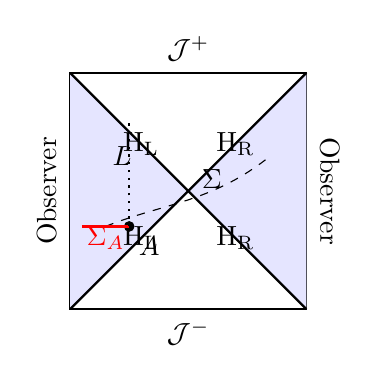
\begin{tikzpicture}[scale=3]
    % Define coordinates
    \coordinate (tl) at (0,1);
    \coordinate (tr) at (1,1);
    \coordinate (bl) at (0,0);
    \coordinate (br) at (1,0);
    
    % Draw the square boundary
    \draw[thick] (tl) -- (tr) -- (br) -- (bl) -- cycle;
    
    % Fill the left and right static patches with light blue
    \fill[blue!10] (tl) -- (0.5,0.5) -- (bl) -- cycle;
    \fill[blue!10] (tr) -- (0.5,0.5) -- (br) -- cycle;
    
    % Draw the horizons
    \draw[thick] (tl) -- (br);
    \draw[thick] (tr) -- (bl);
    
    % Label the horizons
    \node at (0.3,0.7) {$\mathrm{H_L}$};
    \node at (0.7,0.7) {$\mathrm{H_R}$};
    \node at (0.3,0.3) {$\mathrm{H_L}$};
    \node at (0.7,0.3) {$\mathrm{H_R}$};
    
    % Draw and label the spacelike slice
    \draw[dashed] (0.15,0.35) .. controls (0.4,0.45) and (0.6,0.45) .. (0.85,0.65);
    \node at (0.6,0.55) {$\Sigma$};
    
    % Draw and label point A
    \filldraw (0.25,0.35) circle (0.02) node[below right] {$A$};
    
    % Draw the segment Sigma_A
    \draw[red, thick] (0.05,0.35) -- (0.25,0.35);
    \node[red] at (0.15,0.3) {$\Sigma_A$};
    
    % Draw the future lightsheet
    \draw[dotted, thick] (0.25,0.35) -- (0.25,0.8);
    \node at (0.22,0.65) {$L$};
    
    % Label the observers and boundaries
    \node[rotate=90] at (-0.1,0.5) {Observer};
    \node[rotate=270] at (1.1,0.5) {Observer};
    \node at (0.5,1.1) {$\mathcal{J}^+$};
    \node at (0.5,-0.1) {$\mathcal{J}^-$};
    
\end{tikzpicture}

\end{document}